% !Mode:: "TeX:UTF-8" 

\BiChapter{克隆代码创建时一致性维护需求预测方法}
{Predicting Clone Consistency-Requirement at Clone Creating Time}

\BiSection{引言}
{Introduction}

由于日益增长的软件开发的需求,开发人员在软件开发过程中通过一些技术手段,如复制粘贴既有代码,向系统中引入新的克隆代码。新产生的克隆代码会随着系统演化,其演化过程中可能会发生一致性变化。然而,克隆代码的一致性变化不仅会导致系统额外的维护代价,遗忘该一致性变化还会引入与之相关的克隆一致性缺陷,从而将进一步增大系统的维护代价。本文将由复制粘贴操作创建的克隆代码在其演化过程中所发生的一致性变化,称为克隆代码创建时的一致性维护需求。在克隆代码创建时预测克隆代码的一致性维护需求,可以帮助降低系统的维护代价,从而帮助提高软件质量和可维护性。

鉴于此,在定义克隆代码创建时的一致性变化和一致性维护需求的基础上,本章使用机器学习方法在克隆代码创建时预测其一致性维护需求。为训练克隆代码创建时一致性预测模型,首先通过构建软件系统的克隆家系来收集系统中所有的克隆创建实例(复制粘贴导致的克隆代码)。然后,提取了代码属性和上下文属性两组属性值表示克隆代码创建实例。最后,使用机器学习方法训练预测模型,并预测克隆代码创建时的一致性维护需求。在四个开源软件系统上对本章方法进行了评估,实验结果表明本章方法以较高的准确率和召回率高效地预测克隆代码创建时的一致性维护需求。本章所提出的预测方法可以帮助程序开发员在克隆代码创建时预测克隆代码的一致性,降低克隆代码导致的额外的维护代价,从而提高软件的质量和可维护性。

\BiSection{克隆代码创建时一致性维护需求}
{Clone Creating Consistency-Requirement}

\BiSubsection{相关研究}
{Related Work}

在软件开发过程中,通过复制和粘贴操作复用既有代码已经成为一种常见的软件开发手段\cite{koschke2007survey}。复制粘贴活动可以减少软件开发时间和提高软件开发效率,但同时也会向软件系统中创建新的克隆代码(克隆创建)。克隆代码会长时间的存在于软件系统中,并同时随着软件系统进行演化。克隆代码随系统进行演化的过程可以使用克隆家系进行描述\cite{kim2005empirical}(克隆演化见本文~\ref{ref-evolution}~节)。经研究发现在克隆代码的演化过程中,克隆组内的某一克隆代码片段可能会被程序开发人员修改,从而引发克隆代码的变化。同时,由于同组的克隆代码彼此相似,这种变化也可能会传播到同组的其它克隆代码片段中,从而引起克隆组一致性变化\cite{saha2011automatic}。

为了帮助分析克隆代码的变化以及演化情况,本文第二章基于机器学习中的聚类方法挖掘克隆代码的演化特征。研究表明在克隆代码的演化过程中,存在相当数量的克隆代码会发生变化。这些发生变化的克隆代码也会引发克隆组的一致性变化模式。更为重要的是,演化中的克隆代码的一致性变化往往多于不一致性变化,因此在第二章中本文建议程序开发人员需要警惕克隆变化,并且当发生变化时需要考虑克隆代码的一致性问题。(具体可参考本文~\ref{ref-characteristics}~节)

为确保演化中的克隆代码的一致性,程序开发人员需要对发生变化的克隆进行一致性维护,从而导致额外的维护代价。而遗忘克隆的一致性变化,会导致克隆代码的不一致缺陷,从而进一步增加软件的维护代价\cite{aversano2007clones}\cite{bettenburg2009empirical}。本文将在演化过程中由于克隆一致性变化所导致的维护代价称为一致性维护代价。为了避免克隆代码的一致性维护代价,程序开发人员可以在复制粘贴时避免可能发生一致性变化的克隆代码,或者仅允许不会发生一致性变化的克隆代码的产生。换言之,在复制粘贴时预测克隆代码在演化过程中是否会发生一致性变化,可帮助避免一致性维护代价。

\begin{figure}[htbp]
\centering
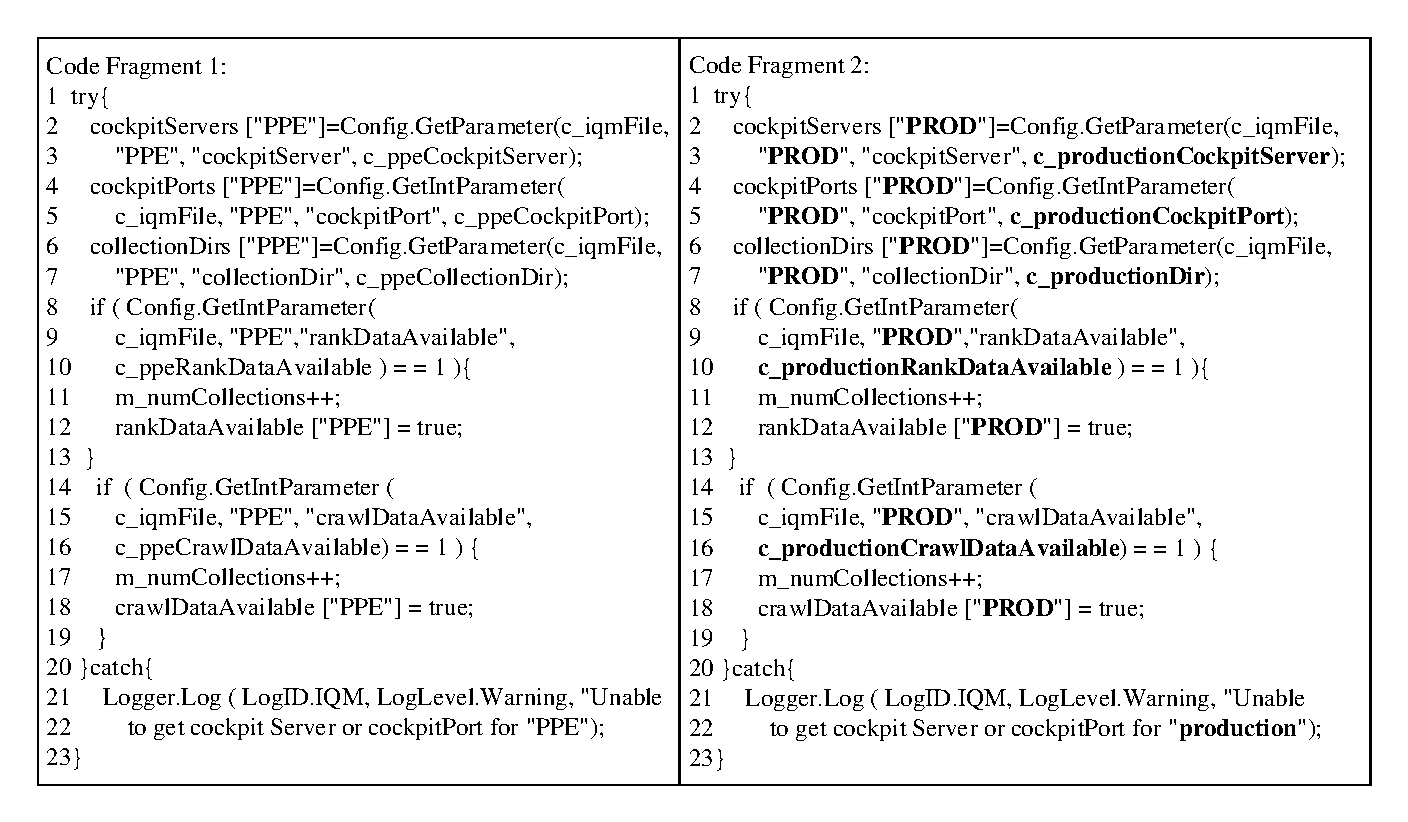
\includegraphics[width = 1.0\textwidth]{creatinga.pdf}
\bicaption[creatingexamplea]{}{导致额外维护代价的克隆代码实例}
{Fig.$\!$}{Two code fragments causing the cost of maintenance}
\vspace{-1em}
\end{figure}

\begin{figure}[htbp]
\centering
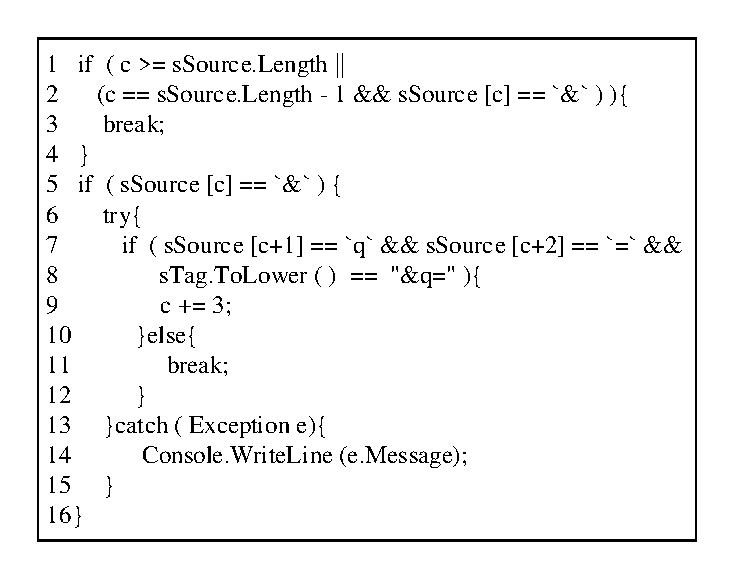
\includegraphics[width = 0.6\textwidth]{creatingb.pdf}
\bicaption[creatingaxampleb]{}{静态的克隆代码实例}
{Fig.$\!$}{Clone Fragment static}
\vspace{-1em}
\end{figure}

因此,Wang等人基于贝叶斯网络在复制粘贴时对克隆代码进行一致性维护需求预测,帮助避免需要一致性维护的克隆代码\cite{wang2012can}\cite{wang2014predicting}。该方法中提取了历史属性、代码属性和上下文属性三组属性表示复制粘贴操作,并使用贝叶斯网络预测克隆代码一致性维护需求。但是,该方法存在以下不足之处:
\begin{itemize}
\item
首先,所使用的历史属性与复制粘贴操作的关联性较弱,仅表示其所在文件的历史变化情况。同时历史属性的提取也增加了方法本身的困难程度(历史属性提取需要分析软件全部版本源代码);
\item
其次,所提取的代码属性和上下文属性不够充分,并不能完全的表示复制粘贴操作所导致的克隆代码。例如,代码属性中仅考虑了克隆代码与系统其它模块的调用和访问关系,并没有详细的考察克隆代码自身的一些属性特征。
\item
最后,方法中没有清晰的给出克隆变化以及一致性维护需求的定义。
\end{itemize}

鉴于此,本章对复制粘贴产生的克隆代码的一致性维护需求,进行了进一步的深入研究。本章在克隆代码演化的基础上结合克隆代码一致性维护,首先给出了一种克隆代码一致性变化以及一致性维护需求的定义,可更为准确地帮助预测克隆的一致性维护需求。然后,本文在Wang等人研究的基础上,改进了克隆代码一致性维护需求预测所使用的度量值。舍弃了与复制粘贴操作关联性不强的历史属性,并进一步扩展了代码属性和上下文属性,可以更为详细和细致的表示由复制粘贴操作导致的克隆代码。最后,使用贝叶斯网络在克隆代码创建时预测其一致性维护需求。本章方法可以帮助程序开发人员降低克隆代码的一致性维护代价,避免克隆一致性缺陷。

%上述不足限制了该方法的实际应用,无法将其应用到具体的软件开发实践中。为解决上述问题,本文对由于复制粘贴产生的克隆代码的一致性维护需求预测进行了进一步研究,在软件开发过程中实现对其的一致性维护需求预测。首先,本文给出新的一致性变化定义,可更为准确地定义和预测克隆的一致性维护需求。然后,在通过构建克隆家系提取复制和粘贴操作后,舍弃历史属性并扩展了代码属性和上下文属性用于表示复制和粘贴操作。然后,本文除使用贝叶斯网络作为预测模型之外,还分析了其它预测模型在克隆代码一致性需求预测问题上的适用性。
%在预测克隆代码的一致性维护需求时,本文有保守模式和激进模式两种使用模式。使用保守模式开发人员可以谨慎的开发软件,通过仅允许不需要一致性维护的复制粘贴操作,从而避免引入会导致额外的克隆代码产生。使用激进模式下开发人员可以快速地开发软件节约开发时间,通过仅阻止需要一致性维护的复制粘贴操作,从而让软件开发人员安全快速的开发软件。本文使用不同的分类器在四个开源软件上进行了实验评估,结果表明本文方法可以同时在保守模式和激进模式下以较高的准确率和召回率对克隆代码进行一致性维护需求预测。本文的主要贡献如下:
%(1)本文定义了新的克隆代码一致性变,并根据其定义了克隆代码的一致性维护需求,可以更为准确的标识克隆代码的一致性维护代价;
%(2)本文使用并扩展代码属性和上下文属性两组属性组,实验结果表明所使用的属性在克隆一致性维护需求的预测中起到了积极的作用;
%(3)本文预测克隆代码的一致性维护需求,不仅在贝叶斯网络分类器上进行了实验评估,还在一般分类器上进行了实验验证,实验结果表明本文方法具有一般性,可以适用于一般的机器学习方法。


%%。本文使用NiCad检测克隆代码(包含Type 1、Type 2和Type 3克隆代码),并使用 {\em Unique Percentage Items (UPI)}来计算克隆片段之间的相似度\cite{roy2008nicad}。



\BiSubsection{克隆创建时一致性维护需求定义}
{The Definitions for Clone Creating Consistency-Requirement}

在克隆代码的演化过程中,克隆片段可能会被开发人员修改,从而导致克隆代码的一致性变化,这种变化可能会导致额外的维护代价。为了描述这种克隆代码的修改,本章给出克隆代码变化时一致性变化定义,如下所示:\\

\begin{definition}
[创建时一致性变化]  
\label{def-creatingchange}
给定两个克隆代码片段 $CF_1$和 $CF_2$,且它们被分别地修改为$CF'_1$和$CF'_2$。如果克隆代码$CF_1$和$CF_2$的变化满足以下条件,称此变化为克隆创建时的一致性变化(Creating Consistent Change), 
  \[
  \begin{array}[t]{cr}
    \mathit{textSim}(CF_i, CF'_i) < 1 & \forall i \in \{1,2\}  \\
  \end{array}
  \]
\end{definition}

%定义2.克隆变化.在版本$V_j$中存在某一克隆组$CG$, $CF$是$G$中某一克隆片段。当克隆演化到$V_{j+1}$版本时,$CF$在中仍存在该克隆组内,记为$CF'$。本文使用$SimText(CF,CF')$表示克隆片段是否发生变化:若$SimText(CF,CF')<1$,则克隆片段发生变化;若$SimText(CF,CF')=1$,则克隆片段未发生变化。其中$SimText(CF,CF')$计算方法与NiCad相同,使用$UPI$计算其相似度。

注意$\mathit {textSim}(CF_i, CF'_i)= 1 - UPI(CF_i, CF'_i)$,UPI是两个代码片段之间不同的代码行数占总代码行的比例。假如给定两个代码片段$CF_1$和$CF_2$,其$UPI(CF_1,CF_2)=0.3$表示两者的差异程度为30\%。同时,其相似度可根据$UPI$计算:$SimText (CF_1,CF_2)=1-UPI=0.7$,表示两者的相似度为70\%。本文在检测克隆代码时,设置克隆代码的相似度阈值为0.7,即相似度大于阈值的代码片段为克隆代码。该定义仅要求克隆代码片段 $ CF_1 $和$CF_2 $被同时修改。

创建时一致性变化,仅要求克隆代码片段被同时的修改。原因在于:在克隆代码创建时,目标是避免新创建的克隆代码在其未来演化过程中的一致性变化,及其所导致额外的维护代价。因此,只要两个克隆片段在其演化过程同时变化,即认为会导致额外维护代价。

克隆创建(复制粘贴操作)所导致的克隆组,会随着系统的演化而演化。在此过程中,组内克隆片段的变化也导致了克隆组的变化,并使用克隆演化模式描述克隆组的变化,称其为一致性变化模式或不一致变化模式。克隆组一致性变化模式定义如下所示:\\
\begin{definition}
[创建时一致性变化模式] 
\label{def-creatingpattern}
在软件版本 $j+1$中存在一个克隆组$CG'$ ,假设克隆组内至少存在两个克隆代码片段$CF'_1$ 和 $CF'_2$可以与映射到上一版本$j$的克隆组$CG$中,且 $CG$中与之对应的克隆代码片段的 $(CF_1,CF_2)$被修改为$(CF'_1,CF'_2)$。如果克隆片段之间的变化( $(CF_1,CF_2)$变化至$(CF'_1,CF'_2)$满足克隆片段的“一致性变化(Consistent Change)”,则称克隆组$CG'$具有一致性变化模式(Consistent Change Pattern)。
\end{definition}

%定义3.一致性变化模式.克隆组$CG$从版本$V_j$到$V_j+1$演化为$CG'$。假如$CG$中至少存在两个克隆代码片段$(CF_1,CF_2)$同时发生了变化,记为$(CF'_1,CF'_2)$。如果$CF'_1$和$CF'_2$同时满足$SimText(CF_1,CF'_1)<1$且$SimText(CF_2,CF'_2)<1$,称克隆组$CG$在演化为$CG'$时发生一致性变化模式,反之称为不一致变化模式。

本章定义的克隆创建时的一致性变化模式,与其它论文中的定义不同。其原因在于:本章目的在于预测克隆代码的一致性所引发的维护代价。为了便于读者更容易理解克隆创建的克隆组的一致性维护需求,本章现给出克隆创建实例的定义,如下所示:\\

\begin{definition}
[克隆创建实例] 
\label{def-creatinginstance}
克隆创建实例:软件版本 $j$中的一个克隆组$CG$是克隆创建实例,如果该克隆组$CG$是其克隆家系$CGE$的根节点。
\end{definition}
%In the above definitions, we identify a $CG$ created by a creating operation (copy and paste) as a new $CGE$ root that begins its evolution. 

%定义1.复制粘贴实例.给定一个克隆组$CG$,其整个演化历史可用克隆家系表示。在表示克隆组$CG$整个演化历史的克隆家系中,第一次出现的克隆组是认为是由复制粘贴活动导致,并称第一次出现的克隆组为复制粘贴实例。


给定一个克隆创建实例所产生的克隆组,在其演化过程中,可能会发生一致性变化模式。克隆组的一致性变化会引发一致性维护代价,从而降低软件质量。因此,在克隆创建时,预测其在演化过程是否会发生一致性变化,可以避免与克隆创建导致的克隆代码的一致性维护代价。本文将创建时克隆代码导致的一致性变化,称为克隆一致性维护需求。克隆创建时的一致性维护需求定义如下:\\

\begin{definition}
[创建时一致性维护需求] 
 \label{def-creatingrequirement}
给定版本 $j$中一个克隆创建实例,$CG$满足克隆一致性维护需求(Consistency-Requirement),如果在版本$k$中存在一个克隆实例 $CG'$($k>j$)满足以下条件: (1) 在$CG'$中至少存在两个克隆片段在其克隆家系$CGE$中可以映射到克隆实例 $CG$中, (2) $CG'$ 具有“一致性变化模式”(Consistent Change Pattern)。反之,假如克隆创建实例$CG$ 不满足克隆一致性维护需求条件,称该克隆实例不需要一致性维护(Consistency-Requirement Free,或者Consistency-Free)。
\end{definition}

%定义4.一致性维护需求.给定一个复制粘贴实例(即克隆组),可以用克隆家系描述其整个演化过程。在其演化过程中,该复制粘贴实例至少发生过一次一致性变化模式,则称该实例满足一致性维护需求。

最终,可以将本章的的研究问题表述如下:给定一个克隆创建实例$CG$,即复制粘贴活动导致的克隆代码,预测创建实例$CG$是否满足克隆创建时的一致性维护需求。

更进一步,根据上述定义克隆创建实例只有两种状态:满足和不满足一致性维护需求。本章克隆创建时的克隆一致性需求预测问题可转换为一个典型的分类问题,因此使用机器学习模型解决此分类问题,具体方法见下文。

\BiSection{克隆代码创建时一致性维护需求预测框架}
{The Framework of Clone Creating Consistency-Requirement Prediction }

为解决本章所提出的克隆一致性需求维护预测问题,本文首先给出了一个方法框架。
基于贝叶斯网络的克隆创建时一致性维护需求预测框架如图~\ref{framwork3}所示。
方法可以划分为三个阶段,克隆创建实例收集阶段、克隆创建实例表示阶段和一致性维护需求预测阶段。收集阶段旨在收集系统中全部的克隆创建实例,可将其用于使用机器学习方法中来训练预测模型。由于实际的克隆创建实例无法直接应用于机器学习方法中,因此在表示步骤中将提取相应的属性值表示克隆创建实例。接下来,在预测步骤,使用属性化的克隆创建实例构建和训练机器学习模型,并使用其预测克隆创建实例的克隆一致性维护需求。

\begin{figure}[htbp]
\centering
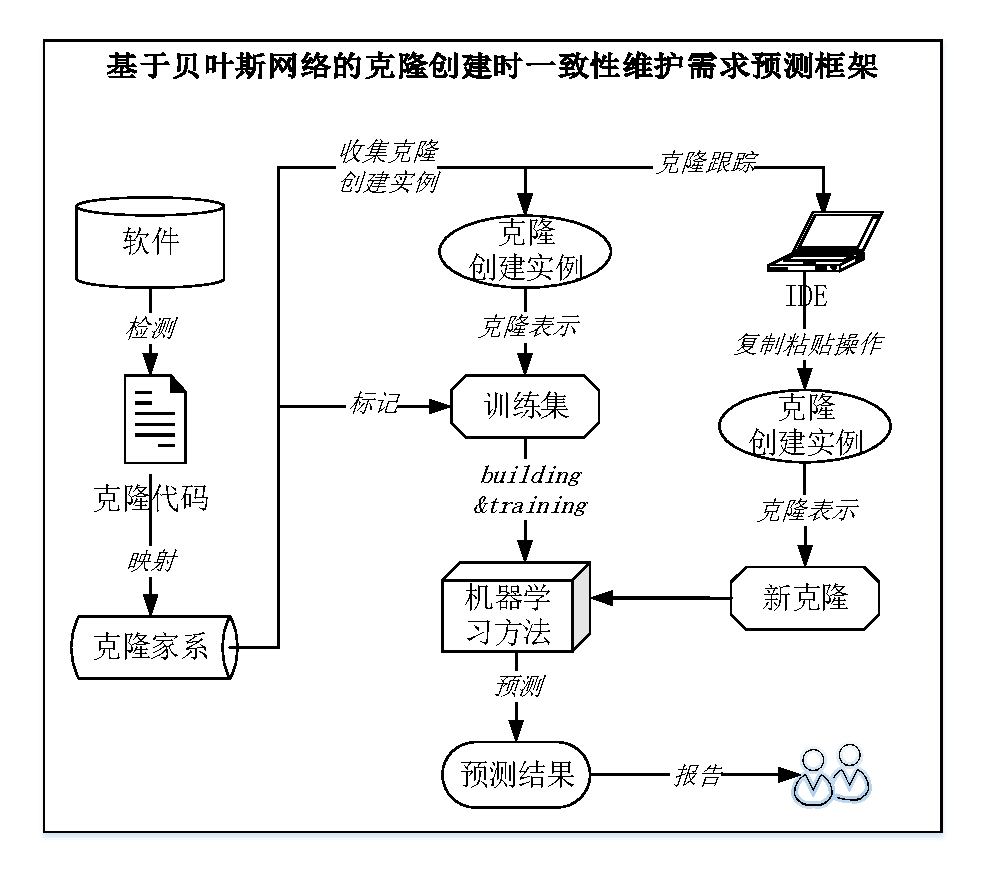
\includegraphics[width = 0.8\textwidth]{framework3.pdf}
\bicaption[framwork3]{}
{克隆创建时一致性维护需求预测框架}
{Fig.$\!$}{The framework for clone creating consistency prediction}
\vspace{-1em}
\end{figure}

具体来说,在收集阶段中,通过构建系统的克隆家系从软件中收集所有的克隆创建实例。使用NiCad来检测软件版本中的所有克隆,并通过在相邻版本的克隆组之间进行映射来构建克隆家系,用于识别克隆创建实例。在表示阶段中,通过提取属性值表示克隆创建实例,提取了代码属性、上下文属性两组属性分别表示被复制和粘贴的克隆代码。在预测阶段中,使用收集到的克隆创建实例训练机器学习模型,并在克隆创建时预测克隆一致性维护需求。在使用已构建好的模型进行预测时,可将该模型嵌入到软件开发环境中。软件开发环境需要实时监测复制粘贴操作(克隆创建实例),然后提取克隆创建实例的度量值。最后,使用模型预测其一致性维护需求,根据预测结果提醒程序开发人员采取进一步的操作。

克隆创建实例有两种不同的预测结果,即满足一致性维护需求和不满足维护需求。
对于满足一致性维护需求实例来说,其在将来的演化中可能会引发一致性变化,程序开发人员可以根据情况选择拒绝此变化实例。对于不满足一致性维护需求实例来说,其在将来的演化中不会引发一致性变化,程序开发人员可以根据情况选择接受此变化实例。

\BiSection{克隆创建实例收集}
{Collecting Clone Creating Instance}
\label{lab-checkcopied}
收集克隆创建实例的目的在于生成克隆一致性预测的训练集,并将其用于训练机器学习模型。通过构建系统的克隆家系并识别其中的克隆演化模式,可以从软件中收集所有的克隆创建实例。首先使用NiCad来检测软件版本中的所有克隆,然后通过在相邻版本的克隆组之间进行映射来构建克隆家系,最后识别克隆一致性演化模式识别系统中的克隆创建实例。

根据定义~\ref{def-creatinginstance}~,本文假定克隆家系$CGE$中第一次出现的克隆代码是由复制粘贴操作导致的,即是克隆创建实例。因此,通过检测系统的克隆代码并构建克隆家系,可以完成对克隆创建实例的收集。

(1)构建克隆家系。首先,下载系统所有版本的源代码,并使用NiCad的默认配置检测检测每一版本的中Type1-3的克隆代码。然后,通过映射所有相邻版本的克隆代码,构建系统中全部克隆家系。为完成版本间的映射,为每个克隆片段生成一个克隆区域描述符 $CRD$\cite{duala2010clone},使用基于$CRD$的克隆映射算法映射两个连续版本之间的所有克隆片段和克隆组\cite{ci2013new}\cite{ci2013newD}。根据克隆映射结果,构建系统的克隆家系。

(2)收集克隆创建实例并标识一致性维护需求。克隆家系是克隆演化的有向无环图,图中根节点是由复制粘贴操导致的克隆创建实例。因此,根据定义~\ref{def-creatinginstance}~通过遍历克隆家系的根节点,可收集系统中所有的克隆创建实例。在收集克隆创建实例的时候,同时根据定义~\ref{def-creatingchange}~和~\ref{def-creatingpattern}~识别克隆一致性变化模式,从而确定克隆创建实例在其未来演化过程发生的一致性变化。根据定义~\ref{def-creatingrequirement}~,如果克隆创建实例在其演化过程中发生了一致性变化模式(~\ref{def-creatingpattern}~),则该实例满足一致性维护需求,否则不满足维护需求。

(3)确认复制和粘贴代码。在收集克隆变化实例后,还需确认该实例中的被复制和被粘贴代码。由于被复制代码会较早地存在软件中,可将创建实例中的克隆代码向上一软件版本中进行映射。假定被复制代码会应存在于上一版本中,被粘贴代码不存在上版本中。根据映射结果,可能会存在两种情况:(a)其中一个克隆代码可以映射,另一个未映射。认为映射代码为被复制代码,未映射为被粘贴代码。(b)两者均没有映射。此情况下随机选取一个为被复制代码,另一个未未被粘贴代码。原因是两者互为克隆代码,彼此之间相似,故随机选取一个为被复制代码并不影响预测结果。注意不存在两者均可映射的情况,应在上一版本检测为克隆代码。\footnote{幸运的是,大多数克隆组只有两个克隆片段,所以这个决定不会影响我们的克隆预测。对于具有多个克隆片段的克隆组,则随机选取两个作为克隆创建实例。}

\BiSection{克隆创建实例表示}
{Representing Clone Creating Instance}
\label{lab-creatingattribute}

本章使用贝叶斯网络预测克隆代码创建时的一致性维护需求,并使用软件中既有的克隆创建实例训练贝叶斯网络模型。但是,实际的克隆创建实例无法直接应用于贝叶斯网络中。因此,本文将提取相应的属性值表示克隆创建实例。将分别提取代码属性、上下文属性两组属性代表克隆创建实例中被复制和粘贴的克隆代码。

%%%代码属性是,上下文属性是,,,,

(1)代码属性

代码属性表示了被复制的克隆代码,从代码自身角度提取被复制克隆代码的特征。代码属性描述克隆代码的词法、语法、函数调用等信息。代码属性主要包括克隆代码粒度、Halstead属性、结构属性、调用属性等,具体的代码属性如下所示:
%部分代码属性源于Wang的工作,本文在其基础上进行了扩展,新增Halstead度量属性、结构属性等。Halstead属性经常用于软件预测中,是用于描述代码特征的度量。结构属性是从代码的语法结构信息。
\begin{itemize}
\item 
克隆粒度:
被复制克隆代码的规模,即所包含的代码行数。
\item 
Halstead属性:
被复制克隆代码的代码复杂度,有四个基本的属性值,分别为操作符种类、操作数种类、操作符总量和操作数总量。
\item  
结构属性:
被复制克隆代码的结构特征,是语句的统计信息,\verb+if_then+, \verb+if\_else+, \verb+switch+, \verb+while+, \verb+do+, \verb+for+,  \verb+this\_or\_super+等。
\item  
参数访问数量:
被复制克隆代码中所有函数的参数访问数量统计。
\item  
总函数调用次数:
被复制克隆代码中所有函数调用的次数统计。
\item  
本地函数调用次数:
被复制的克隆代码中,调用函数与被复制克隆片段在相同类的调用次数统计。
\item  
库函数调用次数:
被复制的克隆代码中,库函数的调用次数统计,包括java库函数的调用、eclipse库函数的调用以及第三方包函数的调用。
\item  
其它调用次数:
被复制的克隆代码中,既不是库函数调用、也不是本地函数调用的其它调用次数统计,如同项目内其它包函数调用或同包内其它类中的函数调用。
\end{itemize}

(2)上下文属性

上下文属性是被复制和被粘贴代码之间的关系属性,描述了两者之间的克隆关系。上下文属性包括代码相似度、克隆分布、被复制和被粘贴代码之间的一些相似度等等。
%部分上下文属性来自Wang的工作,同时本文也进行了扩展,新增代码相似度、参数类型相似度和块信息标识等属性。
具体的上下文属性如下所示:

\begin{itemize}
\item
代码相似度:
被复制与被粘贴的克隆代码之间的相似度,计算方法和NiCad相同,即UPI\cite{roy2008nicad}。
\item
局部克隆标识:
被复制及粘贴的克隆代码片段是否在同一个文件中。
\item
文件名相似度:
被复制和被粘贴克隆代码所在文件的名相似度。假定文件名分别为$M_1$和$M_2$,则文件名相似度为$Sim(M_1,M_2)$,采用李氏距离\cite{levenshtein1966binary}计算(剩余度量中相似度采用相同方法计算)。
\item
文件名相似度标识:
当克隆是局部克隆时,其文件名相似度为1,为非局部克隆时为0。该属性决定文件名相似度是否起效。
\item
方法名相似度:
被复制和被粘贴克隆代码所在方法的方法名字相似度。
\item
总参数名相似度:
假定被复制和被粘贴克隆代码所在方法为$M$和$N$,计算其参数名相似度之和。假设M和N分别包含m和n个参数,即$(P_1,P_2,…,P_m)$和$(Q_1,Q_2,…,Q_n)$,则总参数名相似度为$Sum(Sim(P_i,Q_j))$。
\item
最大参数名相似度:
假定被复制和被粘贴克隆代码所在方法为M和N,其最大参数名相似度。假设M和N分别包含m和n个参数,即$(P_1,P_2,…,P_m)$和$(Q_1,Q_2,…,Q_n)$,最大参数名相似度为$Max(Sim(P_i,Q_j))$。
\item 
总参数类型相似度:
被复制和被粘贴代码克隆所在方法分别为$M$和$N$,其参数类型相似度之和。假设$M$和$N$分别包含$m$和$n$个参数,其参数类型分别为$(P_1,P_2,…,P_m)$和$(Q_1,Q_2,…,Q_n)$,总参数类型相似度$Sum(Sim(P_i,Q_j))$。
\item
块信息标识:
被复制和被粘贴克隆代码的上下文信息是否相同,相同为$1$,反之为$0$。
\end{itemize}



\BiSection{克隆创建时一致性需求预测}
{Predicting Clone Creating Consistency-Requirement}

本章将克隆代码创建时的一致性维护需求问题,转化成了克隆创建实例的分类问题,即给定一个克隆创建实例,判别其是否满足克隆创建时的一致性维护需求。本文使用机器学习方法对克隆创建实例进行分类,从而预测克隆一致性维护需求。

%%%\BiSubsection{贝叶斯网络方法}
%%%{The Bayesian Network Method}
%%%\label{lab-bayes}
%%%
%%%贝叶斯网络是(Bayesian network)是一种概率图型,可以使用已经观察到的事件来预测将来可能发生的事件\cite{friedman1997bayesian}。贝叶斯网络可以表示成一个有向无环图模型,图中的每一个节点表示一个随机事件,图中的边则表示随机事件发生的条件概率。因此, 贝叶斯网络中的全部节点可以视为一组随机变量{$X_{1},X_{2},...,X_{n}$},贝斯网络的边所有边则可以使用随机变量的条件概率表描述(Conditional Probability Distributions, CPD)。
%%%
%%%一般而言,贝叶斯网络的节点可以是随机变量,可以是可观察到的变量、属性、未知参数等。连接两个贝叶斯网络节点的边则代表两个随机变量之间是非条件独立的,使用事件的条件概率表示。如果两个节点间没有连接,就称其随机变量彼此间为条件独立。条件概率表(CPT)可以描述贝叶斯网络的节点和边的因果关系。
%%%
%%%对克隆代码一致性维护需求预测而言,贝叶斯网络可用来表示克隆创建实例的属性值及其一致性维护需求间的概率关系。克隆创建实例的属性值是贝叶斯网络中的随机事件。给定一个具体的克隆创建实例,可以使用贝叶斯网络计算该实例满足一致性维护需求的概率。

%%%\BiSubsection{训练与预测}
%%%{Training and Predicting}
%%%分成两个小节
%\BiSubsection{构建与训练预测器}
%{Building and Training Predictor}
%\BiSection{一致性预测}
%{Predicting Clone Consistency}

本章没有对机器学习方法进行改进和研究,模型的构建和训练通过调用现有机器学习工具包WEKA完成。WEKA(Waikato Environment for Knowledge Analysis)全称是怀卡托智能分析环境,它是一个Java语言编写的,支持数据挖掘任务的工作平台。WEKA集成了大量能承担数据挖掘任务的机器学习算法,包括数据预处理,分类,聚类,关联规则,特征选择以及可视化功能。

对于每个软件系统,首先,通过收集克隆创建实例并提取相应的属性,用于构建模型训练所需的数据集。然后,调用WEKA中的机器学习算法实现构建和训练克隆一致性预测模型。

根据定义~\ref{def-creatingrequirement}~,克隆创建实例有两种不同的状态:需要一致性维护和不需要一致性维护。因此在进行一致性维护需求预测时,克隆创建实例也具有两种不同的预测结果:
\begin{itemize}
\item 
不需要一致性维护:
若克隆创建实例的预测结果为“不需要”,软件开发人员可以自由的执行克隆创建操作(复制和粘贴),从而节约开发时间提高开发效率。因为,该克隆创建实例,在未来演化的过程中不会引发一致性变化,也不会导致额外的维护代价。
\item
需要一致性维护:
若克隆创建实例的预测结果为“需要”,软件开发人员需要谨慎的执行克隆创建操作(复制和粘贴)。因为,该克隆创建实例,在未来演化的过程中可能会引发一致性变化,从而向系统中引入额外的维护代价。
\end{itemize}

在使用已训练好的模型进行预测时,可以与软件开发过程相结合,将该模型嵌入到软件开发环境中,帮助程序开发人员实现边开发边预测克隆创建实例的一致性维护需求。首先,在软件开发环境中需监测程序员的复制和粘贴操作,识别由此产生的克隆创建实例。然后,根据上文描述的代码和上下文属性,提取相应的特征表示该克隆创建实例。最后,使用训练好的预测器预测该克隆创建实例的一致性维护需求,根据预测结果提醒程序开发人员采取进一步的操作。

\BiSection{实验结果与分析}
{Experiments Results and Analysis}

本节给出本章的实验结果与分析,首先简单介绍了实验所使用的实验系统和评估方法,然后详细给出每个实验的结果与分析。

\BiSubsection{实验系统与实验设置}
{Experimental Projects and Methodology}

为评估本章方法,本章选取了四个开源软件进行实验。四个实验系统的克隆创建实例统计情况如表~\ref{creatingsta}~所示。具体来说,第3列和第4列分别给出了不需要一致性维护和需要一致性维护的克隆创建实例的数量和比例。不需要一致性维护的克隆实例,在其未来的演化中不会导致一致性变化和额外的维护代价。需要一致性维护的克隆实例,在其演化过程中可能导致一致性变化,从而增加系统维护代价。

从表~\ref{copysta}~中可以得出两个发现。第一,软件系统中存在大量的克隆创建实例,数量从633到3366,其中项目 jEdit是含有最少的克隆变化实例。这说明复制粘贴既有代码,已经成为了程序开发人员的一种常用开发手段。第二,软件系统中大部分的克隆创建实例在其演化过程中不满足一致性维护要求(比例从59.8\%到88.47\%)。这表明作为一种常用开发手段的复制粘贴操作并不会在演化中引入一致的变化,这意味着开发人员可以正常的使用这种技术。同时,还可以看出克隆代码在演化过程是比较稳定的,不易发生变化。这与本文第二章得出的克隆演化特征相一致。但是值得注意是:软件系统中依然存在相当数量的需要一致性维护的克隆创建实例,数量从73个到1353个。这也警告程序开发人员,即便可以使用复制粘贴复用已有代码,但也要注意克隆代码的一致性维护问题,不可以肆无忌惮的使用此技术。

\begin{table}[htbp]
\bicaption[copysta]{}{实验系统的克隆创建实例信息统计}
{Table$\!$}{The statistics for clone creating instances in four projects}
\vspace{0.5em}
\centering
\wuhao
\begin{tabular}{cccc}
\toprule[1.5pt]
\multirow{3}{*}{实验系统}& \multicolumn{2}{c}{克隆创建实例的数量(比例)} & \multirow{3}{*}{总数}\\
\cline{2-3}
~&{不需要} &{需要} &  ~\\
~&{一致性维护}&{一致性维护}&~ \\
%\multirow{3}{*}{\textbf{Project}}& \multicolumn{2}{c}{\textbf{Number (Percentage) of Creating Instances}} & \multirow{3}{*}{\textbf{Total}}\\
%\cline{2-3}
%&\textbf{Consistency-} &\textbf{Meeting} &  \\
%&\textbf{Requirement Free}&\textbf{Consistency-Requirement}& \\
\midrule[1pt]
ArgoUML&	2574(77.07\%)&	766(22.93\%)&	3340\\
jEdit&	560(88.47\%)&	73(11.53\%)&	633\\
jFreeChart&	2013(59.80\%)&	1353(40.20\%)&	3366\\
Tuxguitar&	1016(71.10\%)&	413(28.90\%)&	1429\\
\bottomrule[1.5pt]
\end{tabular}
\end{table}

本章将对两种类型的克隆创建实例同时进行预测,即不需要一致性维护的和需要一致性维护的。进一步可将实验划分为“一致性维护自由”实验(不需要一致性维护)和“一致性维护需求”实验两个部分(需要一致性维护)。

首先使用贝叶斯网络模型预测克隆创建实例的一致性。然后,还评估了五种不同机器学习方法的预测能力,试图帮助程序开发人员选择一个最优的机器学习模型用于克隆代码创建时的一致性维护需求预测中。

为了全面评估本章提出的方法,在每个实验中还从两个不同的角度进行了实验分析,即全属性实验、属性组实验两个部分。
\begin{itemize}
\item
全属性实验:使用本章提取的所有属性对实验系统进行分析,评估本文方法的预测能力。
\item
属性组实验:分别使用两组不同的属性组对实验系统进行分析,评估所提取的属性组对预测能力的影响。
%%\item
%%交叉验证实验:使用其它系统数据作为训练集训练模型,并使用该模型在新系统上进行实验分析,从而探索模型在应用到新系统的预测能力。
\end{itemize}

\BiSubsection{贝叶斯网络实验}
{Clone Cloning Consistency Free Experiment}

首先在贝叶斯网络模型上进行实验分析。使用开源软件工具WEKA训练和预测贝叶斯网络。在构建贝叶斯网络时,使用K2搜索算法\cite{}建立网络结构,并设置贝叶斯网络最大父节点个数为3,使用{\em  SimpleEstimator}来估计贝叶斯网络的条件概率表。在实验时将克隆创建实例的数据集划分为训练集和测试集,使用训练集训练贝叶斯网络生成预测模型,然后使用测试集评估贝叶斯网络的预测能力。在全属性实验和属性组实验中,对每一个实验系统在数据集上使用十倍交叉验证(10 Cross-Validity\cite{})评估本文方法。

预测时贝叶斯网络会计算克隆创建实例的概率值,表示该实例需要一致性维护需求的概率(在0~1之间,数值接近于1表示需要一致性维护,接近于0表示不需要一致性维护)。针对不同的克隆创建实例,设置了不同的阈值进行实验分析。对于不需要一致性维护的实例,其预测值较小(接近于0),选取阈值为0.01、0.05、0.10、0.15和0.20,当预测值小于等于给定阈值时认定该实例不需要一致性维护。对于需要一致性维护的实例,其贝叶斯网络预测值较大(接近于1),选取阈值为0.5、1.6、0.7、0.8和0.9,当预测值大于等于该阈值认定该实例需要一致性维护。


\BiSubsubsection{一致性维护自由实验}
{Clone Cloning Consistency Free Experiment}

本实验对不需要一致性维护的克隆创建实例进行预测评估。将关注不需要一致性维护的克隆实例,从而让程序开发人员重点更加放心的执行复制和粘贴操作,从而快速安全的开发软件。此实验使用三个度量评估预测效果,分别为:推荐率、准确率和召回率。
\begin{itemize}
\item	
推荐率(Recommendation Rate):指的是所推荐的不需要一致性维护的克隆创建实例比例,即预测为不需要一致性维护的克隆创建实例与系统中全部实例的比值。
\item  
精确率(Precision):指所预测的不需要一致性维护复制粘贴实例的准确率,即在预测为不需要一致性维护的复制粘贴实例中,正确预测的实例与所预测实例的比值。
\item  
召回率(Recall):指所推荐的不需要一致性维护的复制粘贴实例的查全率,即预测为不需要一致性维护的复制粘贴实例,与系统中的不需要一致性维护的实例的比值。
\end{itemize}

%%%\BiSubsubsection{全属性实验}
%%%{Effectiveness Experiment}
(1)全属性实验

全属性实验使用全部属性在四个实验系统上进行评估,实验结果如表~\ref{copyallfree}~所示。由表中可以看出,本文方法在预测不需要一致性维护的克隆创建实例时,在四个系统上均取得了较好效果。根据预测结果,四个系统的准确率介于86.6--97.22\%之间,同时召回率也达到较高值,介于76.97--96.39\%之间。由表~\ref{copyallfree}~和表~\ref{copysta}~中可以看出,本文的推荐率达到了一个合理的水平, 和系统中不需要一致性维护的克隆实例比例相差不大。同时,阈值对预测结果的影响不大,准确度会随着阈值的降低而缓慢增大。四个系统在不同的阈值的准确度均较高。因此,本文方法在使用全属性在贝叶斯网络作为分类器时,可以达到一个较好的预测效果。

\begin{table}[htbp]
\bicaption[copyallfree]{}{四个实验系统的全属性组实验效果}
{Table$\!$}{The effectiveness for all attribute on four projects}
\vspace{0.5em}
\centering
\wuhao
\begin{tabular}{ccccc}
\toprule[1.5pt]
{系统}&{阈值}&{推荐率(\%)}&{准确率(\%)}&{召回率(\%)}\\
%\textbf{Project}&\textbf{Threshold}&\textbf{RR(\%)}&\textbf{Precision(\%)}&\textbf{Recall(\%)}\\
\midrule[1pt]
\multirow{5}{*}{ArgoUML}
&0.01&	74.61&	95.91&	92.85\\
&0.05&	76.83&	95.21&	94.91\\
&0.1&	77.63&	94.83&	95.53\\
&0.15&  78.26&	94.68&	96.15\\
&0.2&	78.47&	94.66&	96.39\\
\hline
\multirow{5}{*}{jEdit}
&0.01&	73.93&	97.22&	81.25\\
&0.05&	78.67&	95.98&	85.36	\\
&0.1&	80.73&	95.11&	86.79	\\
&0.15&	81.67&	94.97&	87.68	\\
&0.2&	82.15&	94.62&	87.86	\\
\hline
\multirow{5}{*}{jFreeChart}
&0.01&	54.69&	92.40&	84.50\\
&0.05&	57.22&	91.23&	87.28\\
&0.1&	59.24&	89.72&	88.87\\
&0.15&	60.22&	89.15&	89.77\\
&0.2&	61.14&	88.87&	90.86\\
\hline
\multirow{5}{*}{Tuxguitar}
&0.01&	61.51&	88.96&	76.97\\
&0.05&	66.83&	87.96&	82.68\\
&0.1&	69.28&	87.47&	85.24\\
&0.15&	70.82&	86.96&	86.61\\
&0.2&	72.08&	86.60&	87.80\\
\bottomrule[1.5pt]
\end{tabular}
\end{table}

%%%\BiSubsubsection{属性组实验}
%%%{Attribute Set Experiment}
(2)属性组实验

本章提取了两组度量表示克隆创建实例,分别为代码属性和上下文属性。为确定每一组属性对预测效果的作用,本节对每一属性组进行了评估,即属性组实验。在本实验中每次仅使用一组度量去预测实例的一致性维护需求,并观察其对预测结果的影响。实验结果如表~\ref{copysetfree}~所示,其中左侧为代码属性,右侧为上下文属性。

由表~\ref{copysetfree}~和表~\ref{copyallfree}~中可以看出,代码属性实验的预测效果依然较好,但和全属性实验对比发现代码属性实验的召回率下降,准确率除jEdit中少数几个之外也全部下降,因此本文提取的代码属性对预测作用具有积极意义。在上下文属性实验中,预测结果除jEdit系统外准确率提高,但是系统的召回率却大大降低。因此,下上下文属性对系统的准确率影响较大,而代码属性对系统的召回率影响较大,同时两者对于预测都起到了积极的作用。

因此,本文建议在进行预测时,保留所有的属性作为最终的属性,因为某些属性可能对其它尚未验证的系统具有积极的意义。

\begin{table}[htbp]
\bicaption[copysetfree]{}{在四个实验系统上属性组实验结果}
{Table$\!$}{The effectiveness for attribute set on four projects}
\vspace{0.5em}
\centering
\wuhao
\begin{tabular}{cccccccc}
\toprule[1.5pt]
\multirow{2}{*}{实验系统}&\multirow{2}{*}{阈值}&\multicolumn{3}{c}{代码属性(\%)}&\multicolumn{3}{c}{上下文属性(\%)}\\
&&推荐率&精确率&召回率&推荐率&精确率&召回率\\
%\multirow{2}{*}{\textbf{Project}}&\multirow{2}{*}{\textbf{Threshold}}&\multicolumn{3}{c}{\textbf{ Code(\%)}}&\multicolumn{3}{c}{\textbf{ Context(\%)}}\\
%&&\textbf{RR}&\textbf{Precision}&\textbf{Recall}&\textbf{RR}&\textbf{Precision}&\textbf{Recall}\\
\midrule[1pt]
\multirow{5}{*}{ArgoUML}
&0.01&	70.75&	95.64&	87.80&	47.31&	98.10&	60.22\\
&0.05&	73.53&	95.07&	90.71&	61.74&	96.99&	77.70\\
&0.1&	74.82&	94.60&	91.84&	69.22&	96.24&	86.44\\
&0.15&	75.93&	94.32&	92.93&	71.53&	95.90&	89.01\\
&0.2&	76.59&	94.02&	93.43&	73.59&	95.52&	91.22\\
\hline
\multirow{5}{*}{jEdit}
&0.01&	72.20&    96.94&	79.11&	32.95&	99.10&	54.60\\
&0.05&	76.30&	96.48&	83.21&	42.19&	97.25&	68.60\\
&0.1&	78.67&	95.78&	85.18&	47.74&	95.02&	75.86\\
&0.15&	80.09&	95.66&	86.61&	52.55&	93.95&	82.56\\
&0.2&	81.36&	94.76&	87.14&	54.10&	93.36&	84.45\\
\hline
\multirow{5}{*}{jFreeChart}
&0.01&	39.69&	90.94&	60.36&	32.95&	99.10&	54.60\\
&0.05&	43.94&	87.96&	64.63&	42.19&	97.25&	68.60\\
&0.1&	46.70&	86.32&	67.41&	47.74&	95.02&	75.86\\
&0.15&	48.07&	86.16&	69.25&	52.55&	93.95&	82.56\\
&0.2&	48.66&	85.71&	69.75&	54.10&	93.36&	84.45\\
\hline
\multirow{5}{*}{Tuxguitar}
&0.01&	56.75&	89.15&	71.16&	29.60&	93.14&	38.78\\
&0.05&	64.52&	86.98&	78.94&	43.88&	92.34&	56.99\\
&0.1&	67.88&	86.80&	82.87&	51.99&	92.46&	67.62\\
&0.15&	69.56&	86.62&	84.74&	56.54&	91.58&	72.83\\
&0.2&	71.24&	86.05&	86.22&	59.69&	91.56&	76.87\\
\bottomrule[1.5pt]
\end{tabular}
\end{table}


\BiSubsubsection{一致性维护需求实验}
{Clone Creating Consistency-Requirement Experiment}

在本节中,对需要一致性维护的克隆创建实例进行评估。将关注需要一致性维护的克隆实例,由于其在演化过程中可能会引发一致性变化,因此需要警告程序开发人员谨慎的执行复制和粘贴操作,避免额外的维护代价。实验同样使用三个度量对方法进行评估:警告率、准确率和召回率:

\begin{itemize}
\item	
警告率(Warning Rate):指所警告的需要一致性维护的克隆创建实例,即预测为需要一致性维护的实例({$N_1$})与系统中全部实例({$N$})的比值。这些克隆实例可能会引发一致性变化和额外维护代价。警告率为((Warning Rate))计算如下,
%%\[
%%\mbox{\it Warning Rate} ~=~ {\frac {N_1}{N}}
%%\]

\item	
准确率(Precision):指警告为需要一致性维护的克隆创建实例的准确率,即在所预测的需要一致性维护的实例中,正确预测的实例({$TP_1$})与全部警告实例( {$N_1$})的比值。准确率(Precision)计算如下:
%%\[
%%\mbox{\it Warning Rate} ~=~ {\frac {TP_1}{N_1}}
%%\]
%%\item	
召回率(Recall):指所警告的需要一致性维护的克隆创建实例的召回率,即预测为需要一致性维护的实例与系统中的需要一致性维护实例的比值。
\end{itemize}

%%%\BiSubsubsection{全属性实验}
%%%{Effectiveness Experiment}

(1)全属性实验

全属性实验同样使用全部属性在四个实验系统上进行评估,实验结果如表~\ref{copyallmeeting}所示。由表中可以看出,除jEdit外其余系统在不同阈值下取得了可以不错的效果:准确率介于75.79\%--94.94\%之间,召回率介于57.87\%~80.86\%之间。jEdit的预测效果不够理想,其准确度和召回率仅在50\%左右。分析其原因可能为jEdit中训练数据过少导致模型不完全,数据集仅有73复制粘贴实例,仍需要进一步的研究确定。尽管如此,jEdit的预测结果的准确度依然高于其系统自身的一致性维护需求的比例(11.53\%)。因此,在jEdit系统上依然提高了预测的精度,也是有效的。最后,对于四个实验系统,本文所构建的模型均具有有十分合理的警告率,警告率十分接近于满足一致性维护需求的克隆变化实例的比例(如表~\ref {copysta}~中所示)。

虽然阈值的变化可以影响预测的准确率和召回率,但影响并不是十分的剧烈,其中除jEdit对精确率的影响要大于对召回率的影响。尽管如此,在不同的阈值下,本文构建模型的准确率依然达到了较高的水平。因此开发人员可以非常自信地依赖于本文模型的预测结果。然而,本文方法的召回率没有达到准确两率的效果,但仍需进一步增强预测模型的召回能力,这需要进一步的深入研究。

\begin{table}[htbp]
\bicaption[copyallmeeting]{}{四个实验系统全属性的实验效果}
{Table$\!$}{The effectiveness for all attribute sets on four projects}
\vspace{0.5em}
\centering
\wuhao
\begin{tabular}{ccccc}
\toprule[1.5pt]
{实验系统}&{阈值}&{警告率(\%)}&{精确率(\%)}&{召回率(\%)}\\
\midrule[1pt]
\multirow{5}{*}{ArgoUML}
&0.9&	18.95&	94.94&	78.46\\
&0.8&	19.64&	92.84&	79.50\\
&0.7&	20.03&	91.93&	80.29\\
&0.6&	20.24&	91.27&	80.55\\
&0.5&	20.54&	90.23&	80.81\\
\hline
\multirow{5}{*}{jEdit}
&0.9&	10.27&	52.31&	46.58\\
&0.8&	12.16&	48.05&	50.68\\
&0.7&	12.80&	46.91&	52.05\\
&0.6&	13.59&	46.51&	54.79\\
&0.5&	14.06&	47.19&	57.53\\
\hline
\multirow{5}{*}{jFreeChart}
&0.9&	34.25&	91.67&	78.12\\
&0.8&	35.03&	90.75&	79.08\\
&0.7&	35.56&	90.31&	79.90\\
&0.6&	36.19&	89.49&	80.56\\
&0.5&	36.57&	88.87&	80.86\\
\hline
\multirow{5}{*}{Tuxguitar}
&0.9&	20.08&	83.28&	57.87\\
&0.8&	21.48&	81.76&	60.77\\
&0.7&	22.74&	79.38&	62.47\\
&0.6&	23.30&	78.38&	63.20\\
&0.5&	24.28&	75.79&	63.68\\
\bottomrule[1.5pt]
\end{tabular}
\end{table}

%%%\BiSubsubsection{属性组实验}
%%%{Attribute Set Experiment}
(2)属性组实验

类似的,对于一致性维护需求实例,表~\ref{copysetmeeting}~给出了属性组实验结果。由表中可以看出,代码属性的实验结果明显不如全属性组实验,但仍在可接受的范围之内,说明代码属性对预测有积极的影响。上下文属性实验中,当仅仅使用上下文属性时部分系统的实验效果要优于全属性组实验,而部分系统的结果不如全属性组实验。因此,上下文属性对不同的系统所起到的作用并非一样的。上下文属性和代码属性都具有积极地意义,而上下文属性的影响更大。

\begin{table}[htbp]
\bicaption[copysetmeeting]{}{在四个实验系统上属性组实验效果}
{Table$\!$}{The effectiveness for attribute set on four projects}
\vspace{0.5em}\centering\wuhao
\begin{tabular}{cccccccc}
\toprule[1.5pt]
\multirow{2}{*}{系统}&\multirow{2}{*}{阈值}&\multicolumn{3}{c}{ 代码属性(\%)}&\multicolumn{3}{c}{上下文属性(\%)}\\
&&{警告率}&{精确率}&{召回率}&{警告率}&{精确率}&{召回率}\\
%\multirow{2}{*}{\textbf{Project}}&\multirow{2}{*}{\textbf{Threshold}}&\multicolumn{3}{c}{\textbf{ Code(\%)}}&\multicolumn{3}{c}{\textbf{ Context(\%)}}\\
%&&\textbf{WR}&\textbf{Precision}&\textbf{Recall}&\textbf{WR}&\textbf{Precision}&\textbf{Recall}\\
\midrule[1pt]
\multirow{5}{*}{ArgoUML}
&0.9&	17.96&	92.67&	72.58&	15.78&	98.10&	67.49\\
&0.8&	18.89&	89.54&	73.76&	16.98&	95.77&	70.89\\
&0.7&	19.67&	87.52&	75.07&	17.51&	94.02&	71.80\\
&0.6&	20.21&	85.93&	75.72&	18.50&	91.59&	73.89\\
&0.5&	20.78&	84.44&	76.50&	19.64&	87.80&	75.20\\
\hline
\multirow{5}{*}{jEdit}
&0.9&	9.48&	55.00&	45.21&	31.91&	96.65&	76.72\\
&0.8&	11.37&	52.78&	52.05&	33.87&	94.47&	79.60\\
&0.7&	13.27&	48.81&	56.16&	34.94&	93.54&	81.30\\
&0.6&	14.22&	45.56&	56.16&	35.89&	92.30&	82.41\\
&0.5&	14.85&	44.68&	57.53&	37.20&	90.97&	84.18\\
\hline
\multirow{5}{*}{jFreeChart}
&0.9&	27.04&	88.90&	59.79&	31.91&	96.65&	76.72\\
&0.8&	28.19&	87.57&	61.42&	33.87&	94.47&	79.60\\
&0.7&	28.85&	86.61&	62.16&	34.94&	93.54&	81.30\\
&0.6&	29.92&	84.61&	62.97&	35.89&	92.30&	82.41\\
&0.5&	30.57&	83.58&	63.56&	37.20&	90.97&	84.18\\
\hline
\multirow{5}{*}{Tuxguitar}
&0.9&	17.91&	82.03&	50.85&	11.06&	93.04&	35.59\\
&0.8&	20.22&	78.55&	54.96&	15.40&	87.27&	46.49\\
&0.7&	21.48&	76.55&	56.90&	20.50&	83.62&	59.32\\
&0.6&	23.02&	74.16&	59.08&	23.30&	80.18&	64.65\\
&0.5&	24.14&	71.88&	60.05&	26.94&	74.81&	69.73\\
\bottomrule[1.5pt]
\end{tabular}
\end{table}

\BiSubsection{机器学习方法对比实验}
{Cross-Project Experiment}

在此实验中,探讨其他机器学习方法是否可以用于克隆一致性要求预测,属性集是否对此预测产生积极或消极的影响?
在每一个实验中,本章使用五种不同的机器学习方法,并同时对需要一致性维护的克隆实例和不需要一致性维护的克隆实例进行预测。
在实验中,使用五种不同的机器学习方法来验证预测帮助程序开发人员选择合适的机器学习模型。值得注意的是,本文没有对机器学习方法本身做进一步的改进。在培训这五种型号时,必须进行一些设置。大多数这些设置默认设置在WEKA中,无需进一步调整。这意味着有可能进一步增强这些方法的有效性的机会。在我们的实验中,例如,{\ em BayesNet}被训练为克隆创建实例的父节点数设置为3,克隆更改为4。 {\ em Native}只有一个父节点。这两个模型都使用0.5作为两个一致性标签的阈值 - 默认设置为{\ em WEKA}。对于{\ em SVM \ /}方法,我们使用{\ em多项式内核\ /}作为内核函数。对于{\ em Tree \ /},我们使用具有0.75置信因子的J48算法。在{\ em KNN \ /}中,我们使用欧几里德距离作为距离函数与1个邻居进行预测。

在实验中,首先,将数据集分为10个数据集作10倍交叉验证,用于评估预测效果。然后,分别计算满足一致性维护需求和不满足一致性维护需求的准确率(Precision)、召回率(Recall)和F值(F-measure),用于评估不同类型实例的预测效果。最后,将这两组预测结果进行加权平均,使用平均准确率(Average Precision)、平均召回率(Average Recall)和平均F值(Average F-measure)作为指标评估不同机器学习方法的预测能力。

\begin{itemize}
\item
{平均准确率:} 该指标评估克隆实例一致性维护需求预测的准确程度,包含了满足和不满足一致性维护需求的实例。首先,计算预测中满足一致性维护需求的克隆实例的准确率``$P_1$'',即预测为满足一致性维护需求的克隆实例中正确预测的数量与全部预测数量的比值。然后,相似的计算不满足一致性维护需求克隆实例的准确率``$P_2$''。最后,将这两个值进行加权平均,作为整个模型的准确率。 ``$P_1$'' 是满足一致性维护需求的准确率,并且训练集中所有满足一致性的实例数量为``$N_1$'' ;类似地, ``$P_2$''为不满足一致性维护需求的准确率,且 ``$N_2$''为实例数量。平均准确率(Average Precision)计算如下,
\[
\mbox{\it Ave-Precision} ~=~ {\frac {P_1 \times N_1 + P_2 \times N_2}{N_1 + N_2}}
\]

\item
{平均召回率:} 该指标评估克隆实例一致性维护预测的查全能力,包含了满足一致性维护需求和不满足一致性维护需求的实例。同准确率,分别计算满足和不满足一致性维护需求的实例的召回率,然后对两者进行加权平均。$R_1$'' 是满足一致性维护需求的召回率,并且训练集中所有满足一致性的实例数量为``$N_1$'' ;类似地, ``$R_2$''为不满足一致性维护需求的召回率,且 ``$N_2$''为实例数量。平均召回率(Average Recall)计算如下,
\[
\mbox{\it Ave-Recall} ~=~ {\frac  {R_1 \times N_1 + R_2 \times N_2}{N_1 + N_2}}.
\]

\item
{平均F值):} 该指标可以评估所有克隆实例的准确率和召回率的平均有效性。相似地,先分别计算满足和不满足一致性维护需求的克隆实例的F值,然后根据实例的数量进行加权平均。给定一个预测的准确率为precision、召回率为 recall,则该预测的F-Measure可计算如下,
\[  
\mbox{\it F-measure} =2 \times {\frac {\mbox{\it precision} \times \mbox{\it recall} }{ \mbox{\it precision} + \mbox{\it recall} } }
\]
为计算本章预测的平均F-measure, ``$F_1$'' 是满足一致性维护需求的克隆实例的F值,且实例的个数为``$N_1$'';``$F_2$'' 是不满足一致性维护需求的克隆实例的F值,且实例的个数为``$N_1$'',则平均F值(Average F-measure) 可计算如下,
\[
\mbox{\it Ave-F-measure} ~=~ {\frac  {F_1 \times N_1 + F_2 \times N_2}{N_1 + N_2}}.
\]
\end{itemize}

我们采用五种不同的机器学习方法来预测这四个项目的克隆创建时的克隆代码的一致性维护需求,实验结果如表\ref{creatingallavg}~和~\ref{creatingsetavg}~所示。

%\begin{table}[htbp]
%\bicaption[creatingallfree]{}{克隆创建实例的一致性维护自由的预测效果}
%{Table$\!$}{The Effectiveness of Creating Instances for Consistency-Free}
%\vspace{0.5em}
%\centering
%\wuhao
%\begin{tabular}{cccccc}
%\toprule[1.5pt]
%{\textbf{Metric}}&{\textbf{Method}}&{\textbf{ArgoUML}}&{\textbf{jEdit}}&{\textbf{jFreeChart}}&{\textbf{Tuxguitar}}\\
%\midrule[1pt]
%\multirow{5}{*}{Percision}
%&{BayesNet	}&0.945	&0.943	&0.879	&0.861\\
%&{Natvie	}&0.917	&0.941	&0.863	&0.853\\
%&{SVM}&	0.955	&0.919	&0.889	&0.872\\
%&{KNN}&	0.96	&0.933	&0.905&	0.891\\
%&{J48}&	0.953&	0.936	&0.891	&0.913\\
%\hline
%\multirow{5}{*}{Recall}
%&{BayesNet}&	0.974&	0.916&	0.932	&0.917\\
%&{Natvie	}&0.94&	0.85&	0.927	&0.858\\
%&{SVM}&	0.992	&0.998	&0.959&	0.979\\
%&{KNN}&	0.962&	0.943	&0.93	&0.896\\
%&{J48}&	0.969&	0.959&	0.934&	0.935\\
%\hline
%\multirow{5}{*}{F-Measure}
%&{BayesNet}&	0.959	&0.929&	0.905&	0.888\\
%&{Natvie	}&0.928	&0.893	&0.894	&0.856\\
%&{SVM}&	0.973	&0.957&	0.923	&0.923\\
%&{KNN}&	0.961&	0.938	&0.917	&0.893\\
%&{J48}&     0.961&	0.947	&0.912&	0.924\\
%\bottomrule[1.5pt]
%\end{tabular}
%\end{table}

%\begin{table}[htbp]
%\bicaption[creatingallmeeting]{}{克隆创建实例的一致性维护需求的预测效果}{Table$\!$}
%{The Effectiveness of Creating Instances for Meeting Consistency-Requirement}
%\vspace{0.5em}
%\wuhao
%\centering
%\begin{tabular}{cccccc}
%\toprule[1.5pt]
%{\textbf{Metric}}&{\textbf{Method}}&{\textbf{ArgoUML}}&{\textbf{jEdit}}&{\textbf{jFreeChart}}&{\textbf{Tuxguitar}}\\
%\midrule[1pt]
%\multirow{5}{*}{Percision}
%&{BayesNet}&	0.808	&0.575	&0.809	&0.637\\
%&{Natvie}&	0.714	&0.589	&0.78	&0.637\\
%&{SVM}&	0.845	&0.329	&0.823	&0.646\\
%&{KNN}&	0.864	&0.479	&0.854	&0.731\\
%&{J48}&	0.841	&0.493	&0.831	&0.782\\
%\hline
%\multirow{5}{*}{Recall}
%&{BayesNet}&	0.902	&0.472	&0.889	&0.758\\
%&{Natvie}&	0.78	&0.339	&0.878	&0.646\\
%&{SVM}&	0.969	&0.96	&0.931	&0.927\\
%&{KNN}&	0.872	&0.522	&0.892	&0.74\\
%&{J48}&	0.891	&0.61	&0.894	&0.83\\
%\hline
%\multirow{5}{*}{F-Measure}
%&{BayesNet}&	0.853	&0.519	&0.847	&0.692\\
%&{Natvie}&	0.746	&0.43	&0.826	&0.641\\
%&{SVM}&	0.902	&0.49	&0.873	&0.762\\
%&{KNN}&	0.902	&0.49	&0.873	&0.762\\
%&{J48}&	0.865	&0.545	&0.861	&0.805\\
%\bottomrule[1.5pt]
%\end{tabular}
%\end{table}


\begin{table}[htbp]
\bicaption[creatingallavg]{}{克隆创建实例一致性维护需求平均预测效果}
{Table$\!$}{The Average Effectiveness of Creating Instances for Consistency-Requirement}
\vspace{0.5em}
\centering
\wuhao
\begin{tabular}{cccccc}
\toprule[1.5pt]
{指标}&{方法}&{{ArgoUML}}&{{jEdit}}&{{jFreeChart}}&{{Tuxguitar}}\\
%{\textbf{Metric}}&{\textbf{Method}}&{\textbf{ArgoUML}}&{\textbf{jEdit}}&{\textbf{jFreeChart}}&{\textbf{Tuxguitar}}\\
\midrule[1pt]
\multirow{5}{*}{Percision}
&{BayesNet}&0.935&0.889&0.883&	0.831\\
&{Native}&	0.886&	0.871&	0.869&	0.793\\
&{SVM}&0.958&	0.924&0.906&0.888\\
&{KNN}&	0.94&0.886&0.9&	0.848\\
&{Tree}	&0.939&0.898	&0.893&0.889\\
\hline
\multirow{5}{*}{Recall}
&{BayesNet}& 0.936&	0.877&	0.882&	0.836\\
&{Native}&0.888&0.82&	0.868&0.794\\
&{SVM}& 0.958&0.921&0.904&0.883\\
&{KNN}&0.94&0.889&	0.9	&0.848\\
&{Tree}&0.94	&0.905&	0.892&0.891\\
\hline
\multirow{5}{*}{F-measure}
&{BayesNet}&0.935&0.882&0.881&0.832\\
&{Native}&0.887&	0.84&0.867&0.794\\
&{SVM}&0.957&	0.903	&0.903&0.876\\
&{KNN}&0.94&0.887&	0.9	&	0.848\\
&{Tree}	&0.939&	0.901	&0.892&0.89\\
\bottomrule[1.5pt]
\end{tabular}
\end{table}

表~\ref{creatingallavg}~给出了克隆创建实例的使用全部属性组的预测结果。从表中可以看出,五种不同的机器学习方法均可以高效地预测克隆一致性要求,准确率从79.3\%到95.8\%,召回率从79.4\%到95.8\% ,F值从79.4\%至95.7\%。同时,对比不同机器学习方法的有效性,通过对比发现,SVM在这四个实验系统上具有最佳的预测能力。具体来说,SVM在系统 ArgoUML、jEdit和jFreeChart上有最好的结果。对于{Tuxguitar}系统来说,决策树具有最好的结果,SVM具有第二好的预测结果。与此同时,贝叶斯网络和朴素贝叶斯方法在这四个项目中几乎具有相对较差的预测结果,但是相差并不明显。
因此,建议开发人员在需要预测克隆创建实例时首先考虑SVM,其它的机器学习方法也可以作为选择进行考虑。

\begin{sidewaystable} [htbp]
\bicaption[creatingsetavg]{}{克隆创建实例的属性组平均预测效果}
{Table$\!$}
{The Average Effectiveness of Attribute Set on Creating Instances for Consistency-Requirement}
\vspace{0.5em}
\centering
\wuhao
\begin{tabular}{cccccccccccccc}
\toprule[1.5pt]
\multirow{2}{*}{指标}&\multirow{2}{*}{方法}&\multicolumn{3}{c}{\textbf{ArgoUML}}&\multicolumn{3}{c}{\textbf{jEdit}}&\multicolumn{3}{c}{\textbf{jFreeChart}}&\multicolumn{3}{c}{\textbf{Tuxguitar}}\\
\cline{3-14}
&&\textbf{All}&\textbf{Code}&\textbf{Context}&\textbf{All}&\textbf{Code}&\textbf{Context}&\textbf{All}&\textbf{Code}&\textbf{Context}&\textbf{All}&\textbf{Code}&\textbf{Context}~\\
\midrule[1pt]
\multirow{5}{*}{Percision}
&BayesNet&	0.935&	0.912&	0.917&		0.889&	0.885&	0.83&		0.883&	0.808&	0.903&		0.831&	0.811&	0.843\\
&Native&	0.886&	0.866&	0.877&		0.871&	0.865&	0.832&		0.869&	0.755&	0.873&		0.793&	0.747&	0.824\\
&SVM&	0.958&	0.928&	0.942&		0.924&	0.924&	0.909&		0.906&	0.819&	0.906&		0.888&	0.834&	0.873\\
&KNN&	0.94&	0.911&	0.933&		0.886&	0.903&	0.877&		0.9	&0.808&	0.898&		0.848&	0.806&	0.861\\
&Tree&	0.939&	0.904&	0.93&		0.898&	0.882&	0.876&		0.893&	0.802&	0.891&		0.889&	0.8&	0.881\\
\hline
\multirow{5}{*}{Recall}
&BayesNet&	0.936&	0.914&	0.919&		0.877&	0.869&	0.852&		0.882&	0.803&	0.903&		0.836&	0.817&	0.846\\
&Native&	0.888&	0.868&	0.88&		0.82&	0.836&	0.826&		0.868&	0.752&	0.873&		0.794&	0.756&	0.816\\
&SVM&	0.958&	0.929&	0.943&		0.921&	0.921&	0.918&		0.904&	0.806&	0.904&		0.883&	0.837&	0.874\\
&KNN&	0.94&	0.912&	0.934&		0.889&	0.912&	0.885&		0.9&	0.803&	0.898&		0.848&	0.81&	0.862\\
&Tree&	0.94&	0.905&	0.931&		0.905&	0.896&	0.889&		0.892&	0.796&	0.89&		0.891&	0.807&	0.882\\
\hline
\multirow{5}{*}{F-measure}
&BayesNet&	0.935&	0.912&	0.917&		0.882&	0.876&	0.84&		0.881&	0.797&	0.902&		0.832&	0.811&	0.844\\
&Native&	0.887&	0.867&	0.878&		0.84&	0.848&	0.829&		0.867&	0.741&	0.872&		0.794&	0.75&	0.819\\
&SVM&	0.957&	0.927&	0.941&		0.903&	0.903&	0.907&		0.903&	0.797&	0.903&		0.876&	0.827&	0.869\\
&KNN&	0.94&	0.912&	0.933&		0.887&	0.905&	0.881&		0.9&	0.796&	0.897&		0.848&	0.807&	0.862\\
&Tree&	0.939&	0.904&	0.93&		0.901&	0.887&	0.881&		0.892&	0.788&	0.889&		0.89&	0.802&	0.881\\
\bottomrule[1.5pt]
\end{tabular}
\end{sidewaystable} 

%\begin{sidewaystable} [htbp]
%\bicaption[creatingsetfree]{}{克隆创建实例的属性组克隆一致性维护自由预测效果}{Table$\!$}
%{The Effectiveness of Attribute Set on Creating Instances for Consistency-Requirement Free}
%\vspace{0.5em}
%\centering
%\wuhao
%\begin{tabular}{cccccccccccccc}
%\toprule[1.5pt]
%\multirow{2}{*}{\textbf{Metric}}&\multirow{2}{*}{\textbf{Method}}&\multicolumn{3}{c}{\textbf{ArgoUML}}&\multicolumn{3}{c}{\textbf{jEdit}}&\multicolumn{3}{c}{\textbf{jFreeChart}}&\multicolumn{3}{c}{\textbf{Tuxguitar}}\\
%\cline{3-14}
%&&\textbf{All}&\textbf{Code}&\textbf{Context}&\textbf{All}&\textbf{Code}&\textbf{Context}&\textbf{All}&\textbf{Code}&\textbf{Context}&\textbf{All}&\textbf{Code}&\textbf{Context}~\\
%\midrule[1pt]
%\multirow{5}{*}{Percision}
%&BayesNet&0.945&	0.932	&0.929&		0.943&	0.942	&0.9	&	&0.879	&0.789	&0.898		&0.861	&0.848	0.88\\
%&Native&0.917	&0.907&	0.913	&	0.941	&0.932&	0.906	&	0.863&	0.744&	0.873	&	0.853&	0.809	&0.89\\
%&SVM&0.955&	0.937	&0.945	&	0.919	&0.919&	0.928&		0.889	&0.779&	0.889	&	0.872	&0.843	&0.877\\
%&KNN&0.96	&0.94	&0.947	&	0.933&	0.934	&0.926	&	0.905&	0.787&	0.896	&	0.891&	0.856&	0.9\\
%&Tree&0.953&	0.936	&0.943	&	0.936&	0.923	&0.921&		0.891&	0.778&	0.884	&	0.913	&0.842&	0.907\\
%
%\hline
%\multirow{5}{*}{Recall}
%&BayesNet&0.974	&0.958	&0.969	&	0.916	&0.907&	0.936		&0.932	&0.916	&0.944	&	0.917	&0.905	&0.906\\
%&Native&0.94	&0.924	&0.933&		0.85	&0.879&	0.896		&0.927&	0.892	&0.922	&	0.858	&0.86&	0.845\\
%&SVM&0.992	&0.973&	0.983		&0.998	&0.998&	0.984		&0.959	&0.944	&0.959		&0.979	&0.947	&0.957\\
%&KNN&0.962&	0.946&	0.969	&	0.943	&0.968&	0.945		&0.93&	0.919&	0.937	&	0.896	&0.881&	0.907\\
%&Tree&0.969&	0.941	&0.969	&	0.959&	0.963	&0.957	&	0.934	&0.92&	0.939	&	0.935	&0.897	&0.93\\
%\hline
%\multirow{5}{*}{F-Measure}
%&BayesNet&0.959&	0.945&	0.949	&	0.929	&0.924&	0.918	&	0.905&	0.848	&0.921	&	0.888&	0.875&	0.893\\
%&Native&0.928&	0.915	&0.923	&0.893	&0.904	&0.901		&0.894&	0.811&	0.897	&	0.856	&0.834	&0.867\\
%&SVM&0.973&	0.955&	0.964	&	0.957&	0.957&	0.955	&	0.923&	0.854	&0.923&		0.923&	0.892&	0.915\\
%&KNN&0.961&	0.943&	0.958	&	0.938	&0.951&	0.935		&0.917	&0.848	&0.916&		0.893&	0.868	&0.903\\
%&Tree&0.961&	0.938&	0.956	&	0.947	&0.942&	0.939	&	0.912&	0.843	&0.911&		0.924	&0.868&	0.918\\
%\bottomrule[1.5pt]
%\end{tabular}
%\end{sidewaystable}

%\begin{sidewaystable} [htbp]
%\footnotesize
%\bicaption[sdfj1]{}{克隆创建实例的属性组克隆一致性维护自由预测效果}{Table$\!$}
%{The Effectiveness of Attribute Set for Creating Instances for Meeting Consistency-Requirement}
%\vspace{0.5em}
%\centering
%%\wuhao
%\begin{tabular}{cccccccccccccc}
%\toprule[1.5pt]
%\multirow{2}{*}{\textbf{Metric}}&\multirow{2}{*}{\textbf{Method}}&\multicolumn{3}{c}{\textbf{ArgoUML}}&\multicolumn{3}{c}{\textbf{jEdit}}&\multicolumn{3}{c}{\textbf{jFreeChart}}&\multicolumn{3}{c}{\textbf{Tuxguitar}}\\
%\cline{3-14}
%&&\textbf{All}&\textbf{Code}&\textbf{Context}&\textbf{All}&\textbf{Code}&\textbf{Context}&\textbf{All}&\textbf{Code}&\textbf{Context}&\textbf{All}&\textbf{Code}&\textbf{Context}~\\
%\midrule[1pt]
%\multirow{5}{*}{Precision}
%&BayesNet&	0.902	&0.844	&0.878	&	0.472	&0.447	&0.294	&	0.889	&0.836	&0.91	&	0.758	&0.719	&0.752\\
%&Native&	0.78&	0.728&	0.756	&	0.339	&0.352	&0.266	&	0.878	&0.772	&0.873	&	0.646	&0.593	&0.662\\
%&SVM&	0.969	&0.896	&0.934	&	0.96	&0.96&	0.769	&	0.931	&0.879	&0.931	&	0.927&	0.813	&0.863\\
%&KNN&	0.872	&0.815	&0.888		&0.522	&0.66	&0.5		&0.892	&0.839	&0.9	&	0.74&	0.684	&0.767\\
%&Tree&	0.891	&0.799&	0.885	&	0.61	&0.571	&0.529	&	0.894	&0.837&	0.901	&	0.83	&0.697	&0.817\\
%\hline
%\multirow{5}{*}{Recall}
%&BayesNet&	0.808	&0.765&	0.752		&0.575	&0.575	&0.205	&	0.809&	0.636&	0.841	&	0.637&	0.6	&0.697\\
%&Native&	0.714&	0.68	&0.701	&	0.589	&0.507&	0.288		&0.78	&0.542	&0.8	&	0.637	&0.501	&0.743\\
%&SVM&	0.845&	0.779	&0.808	&	0.329	&0.329&	0.411	&	0.823	&0.601&	0.821	&	0.646	&0.567	&0.671\\
%&KNN&	0.864&	0.798	&0.816	&	0.479	&0.479&	0.425	&	0.854&	0.63&	0.838		&0.731	&0.634&	0.751\\
%&Tree&	0.841&	0.782	&0.803	&	0.493	&0.384&	0.37	&	0.831&	0.61&	0.817	&	0.782	&0.586	&0.765\\
%\hline
%\multirow{5}{*}{F-Measure}
%&BayesNet&	0.853&	0.803&	0.81	&	0.519	&0.503&	0.242	&	0.847&	0.722&	0.874	&	0.692&	0.654&	0.724\\
%&Native&	0.746&	0.703	&0.728		&0.43	&0.416	&0.276	&	0.826	&0.637	&0.835		&0.641	&0.543	&0.7\\
%&SVM&	0.902&	0.834&	0.866&		0.49&	0.49	&0.536	&	0.873&	0.714	&0.873	&	0.762	&0.668&	0.755\\
%&KNN&	0.868&	0.806&	0.85	&	0.5&	0.556	&0.459		&0.873	&0.72	&0.868		&0.736&	0.658	&0.759\\
%&Tree&	0.865&	0.79&	0.842	&	0.545&	0.459&	0.435	&	0.861	&0.706&	0.857	&	0.805	&0.637&	0.79\\
%\bottomrule[1.5pt]
%\end{tabular}
%\end{sidewaystable}

为了探索不同属性组对预测效果的影响,在五个机器学习方法上进行了属性组实验,实验结果如表~\ref{creatingsetavg}~所示。表中“全部”列是全部属性实验结果,属性组实验结果在“代码”列和“上下文”列中。

从这个表中可以看出,属性组实验结果和全部属性组实验结果没有显着差异。这表明所使用的属性组不会对克隆创建时一致性预测产生负面影响。尽管如此,在全部实验结果中,效果最差的实验结果往往出现在属性组的实验结果中,即在仅使用代码属性或仅适用上下属属性预测时。具体来说,对系统ArgoUML、 jFreeChart和 Tuxguitar,其仅使用代码属性进行预测时五种机器学习方法的预测效果最差;而对系统jEdit仅仅使用“上下文” 属性的五种机器学习方法预测效果最差。

最后,分析不同机器学习方法之间的预测能力,可以得出与全属性实验相似的结论,即五种机器学习方法的预测能力相差不大,但SVM方法具有相对最好的预测能力。因此建议程序开发人员在预测时保留所有的属性,并优先选择SVM方法。



\BiSubsection{讨论}
{Discussion}

本节从不同的角度评估了所建立的贝叶斯网络模型的预测能力,同时对不需要一致性维护和需要一致性维护的克隆创建实例进行了一致性预测。实验结果表明,本章所构建的模型法在在一致性维护需求和一致性维护自由的实验上均具有高效地预测能力。同时,本文所提取的代码属性和上下文属性对克隆创建实例的一致性维护需求的预测起到了积极的作用。但在不同系统中的两种使用模式下,所产生的影响程度不一致。%本文建议维护人员可以根据项目需求或者自身需求适当的选择属性从而达到不同的要求目标,但仍需要进一步的实验进行验证。
使用全属性在贝叶斯网络作为分类器时,可以达到一个较好的预测效果,因此建议对预测模型进行完全训练。

根据表~\ref{creatingallavg}~和~\ref{creatingsetavg}~中的实验结果,在克隆代码创建时,五种机器学习方法都可以应用于克隆代码的一致性维护需求预测中,并具有相似的预测能力。另外,其预测能力仍然具有一点差异,SVM似乎拥有相对最佳的预测效果,因此优先推荐使用SVM技术应用在一致性预测中。与此同时,所使用的属性组在预测中起到了积极的作用,建议程序开发人员在预测时保留所有的属性组进行变化时一致性预测。

\BiSection{本章结论}
{Summary of this Chapter}

程序开发人员的复制粘贴操作会向系统中引入克隆代码(称为克隆创建实例),而在其演化过程中,克隆创建实例可能会发生一致性变化而导致额外的维护代价。为帮助程序开发人员避免此类维护代价,本章提出了一个克隆代码创建时一致性维护需求预测方法,在克隆代码创建时预测新创建的克隆代码是否会会引发克隆代码的一致性变化,从而帮助程序开发人员决定是否执行该克隆代码创建操作。通过构建软件系统的克隆家系收集克隆创建实例,并使用其构建和训练克隆一致性预测的贝叶斯网络模型。分别使用不同的属性组表示克隆创建实例,即代码属性表示被复制克隆代码和上下文属性表示被粘贴的克隆代码。对四个开源软件项目进行一致性维护需求和自由实验,从而验证所构建模型的预测能力。实验结果表明本章方法可以以较高的准确率和召回率高效的预测克隆代码的一致性维护需求。此外,所提取的两组属性组在预测中均起到了积极的作用,但是对准确率和召回率可能有不同的影响。同时,交叉验证实验尽管预测效果不如全属性实验,但是在针对克隆创建实例不足的新系统时,仍然可以作为一个不错的选择。%具体地,在全属性实验中,实验结果表明本文方法具有较高的预测效果;属性组实验结果表明所提取的两组属性组在预测中均起到了积极的作用,但是对准确率和召回率有不同的影响,并且也依赖于具体的系统;交叉验证实验结果虽然不如全属性实验,但仍在可接受范围内。因此,本文建议对系统进行一致性需求预测时,优先选用自身数据进行训练,并可以根据不同的系统选择不同的度量值以满足程序开发人员的需求。

%%本文方法还可以方便的集成到软件开发环境中(如eclipse),从而在开发时帮助程序开发人员进行一致性维护需求预测。在未来工作中,将会考虑实现一个预测插件,将本文方法切实的应用到软件开发过程中帮助提高软件质量。在交叉验证实验中,使用本文方法预测新系统时,预测效果仍有很大的提升空间。在未来的研究中,将考虑提取并使用新的属性以适用于交叉验证的预测。将考虑训练一个克隆代码一致性维护需求的一般性模型,使其对所有的系统都具有较高的准确率和召回率,进而将其应用于全新系统的一致性维护需求预测中。
